\section{Methodology}
\label{sec:Methodology}

\subsection{Database}
We have collected 8 POEM videos of length around 40-45 mins each. Total 8000 snapshots are extracted from these videos. The snapshots are cropped to 720 x 930 pixels. Out of these 24 snapshots are annotated with the help of Segment Anything Model (SAM) with 4 classes: \textit{Background, Muscle layer, Mucosal layer, and Electrode}. The annotated snapshots are used to train the model.

\begin{figure}[ht]
    \centering
    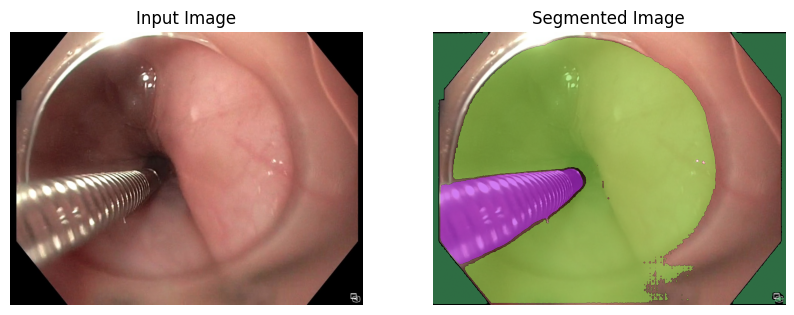
\includegraphics[width=0.4\textwidth]{Images/annoted.png}
    \caption{Annotated image \\ \textit{Background: Green, Muscle layer: Yellow, Electrode: Purple. There is no Mucosal layer in this image.}}
    \label{fig:annotated}
\end{figure}

\subsection{Architecture}

% writing the architecture of the model
A DeepLabv3 model with MobileNetV3 backbone is used. We explain these in detail below.

\subsubsection{DeepLabv3}

DeepLabv3 is a semantic segmentation model that uses Atrous convolution to capture multi-scale context by using different dilation rates. It uses a MobileNetV3 backbone with atrous convolution. The model uses atrous spatial pyramid pooling (ASPP) to capture multi-scale context by using different dilation rates. The model also uses a fully connected conditional random field (CRF) to refine the segmentation results. \\
It takes N feature maps as input from the backbone layer and outputs N*4*H*W tensor, where N is the batch size, 4 is the number of classes, H is the height, and W is the width of the image.The model outputs a probability distribution over the classes for each pixel in the input image.

\begin{figure}[ht]
    \centering
    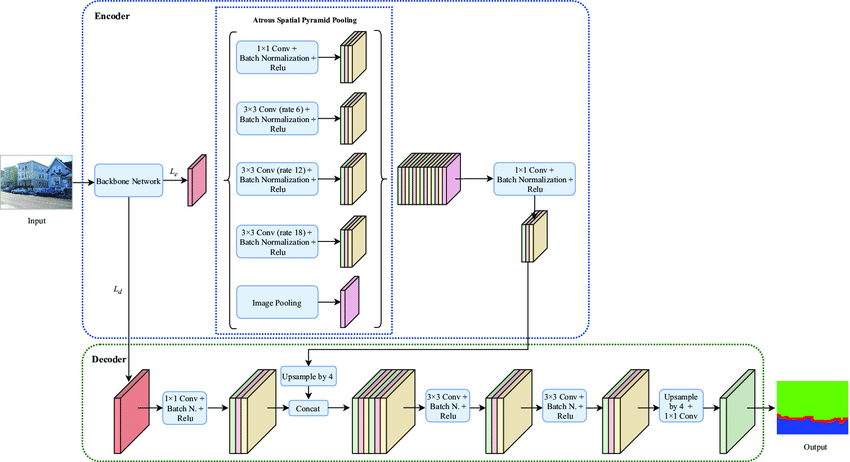
\includegraphics[width=0.53\textwidth]{Images/deeplabv3.png}
    \caption{DeepLabv3 architecture~\cite{deeplabv3-image}}
    \label{fig:deeplabv3}
\end{figure}

\begin{figure}[ht]
    \centering
    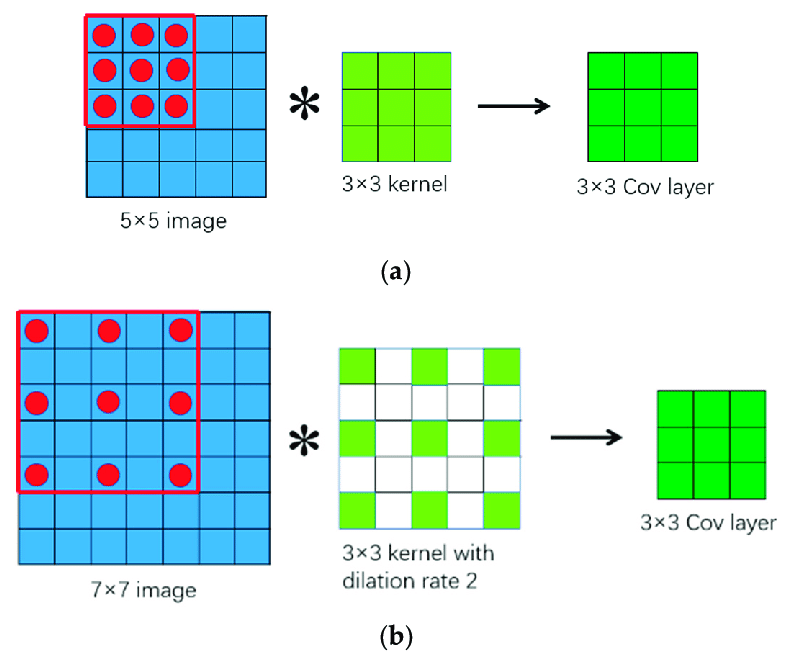
\includegraphics[width=0.5\textwidth]{Images/atrous-convolution.png}
    \caption{Atrous Spatial Pyramid Pooling (ASPP) in DeepLabv3\\ (a) Conv 3x3, rate=1 (b) Conv 3x3, rate=2 \\
    \cite{atrous-convolution-image}}
    \label{fig:atrous-convolution}
\end{figure}


\subsubsection{MobileNetV3-Large Backbone}

MobileNetV3-Large is a convolutional neural network designed for feature extraction. MobileNetV3-Large architecture uses 16 initial filters in the first convolution layer and then reduces the number of filters in the later layers by a factor of 2. It has typically 60 layers. Its building block involves an Inverted Residual Block, which includes a depth-wise convolution, a squeeze-and-excitation module, and a point-wise convolution. It takes normalized RGB images as input and outputs feature maps that are used by DeepLabv3. Input to the layer is a 4-dimensional tensor with normalized RGB channels, and the output is N*32*32, where N is the batch size. It involves downsampling layers.

\begin{figure}[ht]
    \centering
    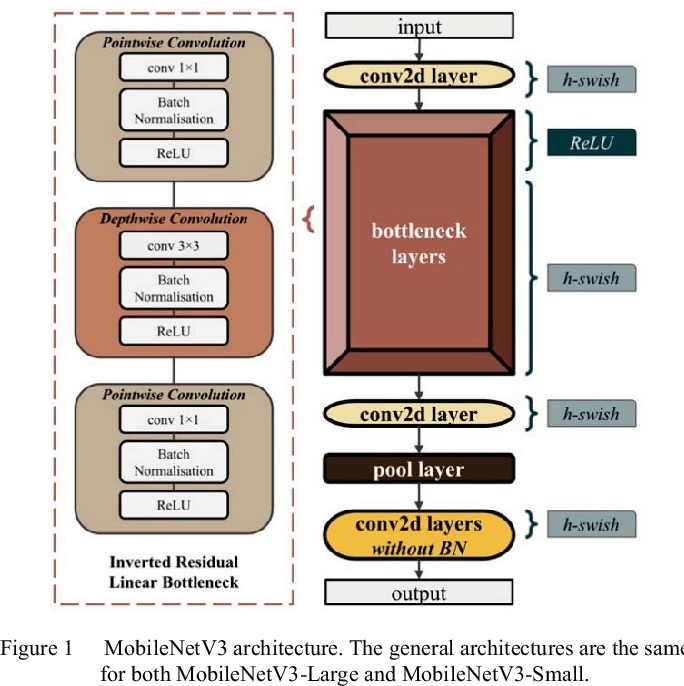
\includegraphics[width=0.5\textwidth]{Images/mobilenet-1.png}
    \caption{\cite{mobilenet-1}}
    \label{fig:mobilenet-1}
\end{figure}

\begin{figure}[ht]
    \centering
    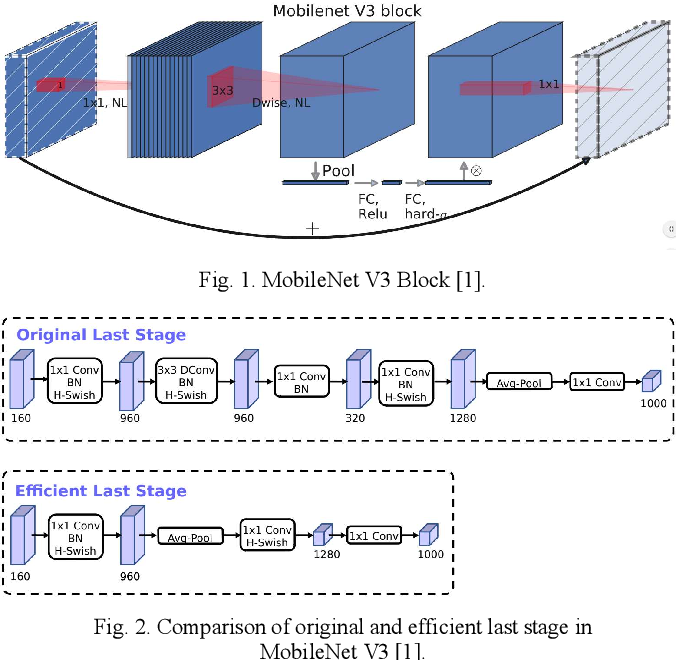
\includegraphics[width=0.5\textwidth]{Images/mobilenet-2.png}
    \caption{\cite{mobilenet-2}}
    \label{fig:mobilenet-2}
\end{figure}

\subsection{Training and Evaluation Setup}
While training on data, the input is a 4-dimensional tensor with normalized RGB channels, and the labels are 2D tensors with integer values representing the class labels for each pixel. The output from the PyTorch model is a 4-dimensional tensor with the shape (N, 4, H, W), where N is the batch size, 4 is the number of classes, H is the height, and W is the width of the output. The output is a probability distribution over the classes for each pixel in the input image. \\
The model is trained with the cross-entropy loss function. We use the Adam optimizer with exponential learning rate schedule with step size of 1 epoch and gamma of 0.8 (Initial Lerning rate = 0.001). Model is trained for 40 epochs with a batch size of 8. The model is trained on 70 images. The model is evaluated on 14 images. The evaluation metrics used are precision, mean intersection over union (mIoU), and pixel accuracy.

\begin{figure}[ht]
    \centering
    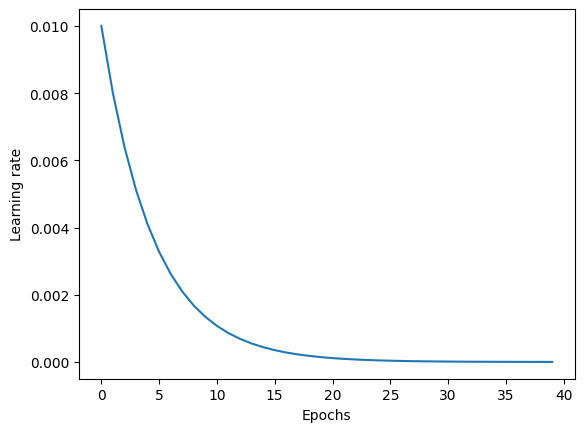
\includegraphics[width=0.5\textwidth]{Images/lr.png}
    \caption{Exponential learning rate schedule}
    \label{fig:lr-schedule}
\end{figure}
